\documentclass{beamer}
\usepackage{amssymb}
\setbeamertemplate{navigation symbols}{}
\setbeamertemplate{footline}[page number]
\usepackage{amsmath}
\usepackage{amsrefs}
\usepackage{graphicx}
\usepackage{bookman}
\usepackage{url}
\usepackage{amsthm}
\usepackage{verbatim}
\usepackage{xcolor}
\bibliographystyle{amsmath}
\usetheme{Madrid}
\usecolortheme{dolphin}
\useoutertheme[footline=authortitle]{miniframes}

%\newtheorem{theorem}{Theorem}[section]
%\newtheorem{corollary}[theorem]{Corollary}

\title[]{Right Whale Recognition}
\author[]{Tyler Allen\\ \footnotesize Clemson University}

\begin{document}

%\setbeamercolor{title}
\begin{frame}
\begin{center}
\maketitle
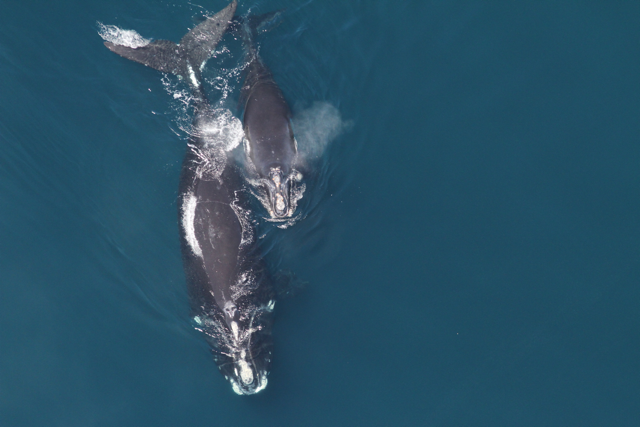
\includegraphics[scale=.5]{title.png}
\end{center}
\end{frame}

\begin{frame}{Motivation}
\begin{itemize}
\item Project from kaggle.com
\item Less than 500 right whales remaining
\item Biologists identify whales by hand
\item Only a few researchers can do this
\end{itemize}
\end{frame}


\begin{frame}{Goals}
\begin{itemize}
\item Data set is photographs of right whales
\item Problem 1: Find right whales
\item Problem 2: Match whale to identification number
\end{itemize}
\end{frame}

\begin{frame}{Strategy Overview}
\begin{itemize}
\item Use photo recognition to find whales
\item Crop found whales from photos
\item Use various algorithms to identify
\end{itemize}
\end{frame}

\section{Recognition}
\subsection{Recognition}
\begin{frame}{Data Example}
\begin{figure}
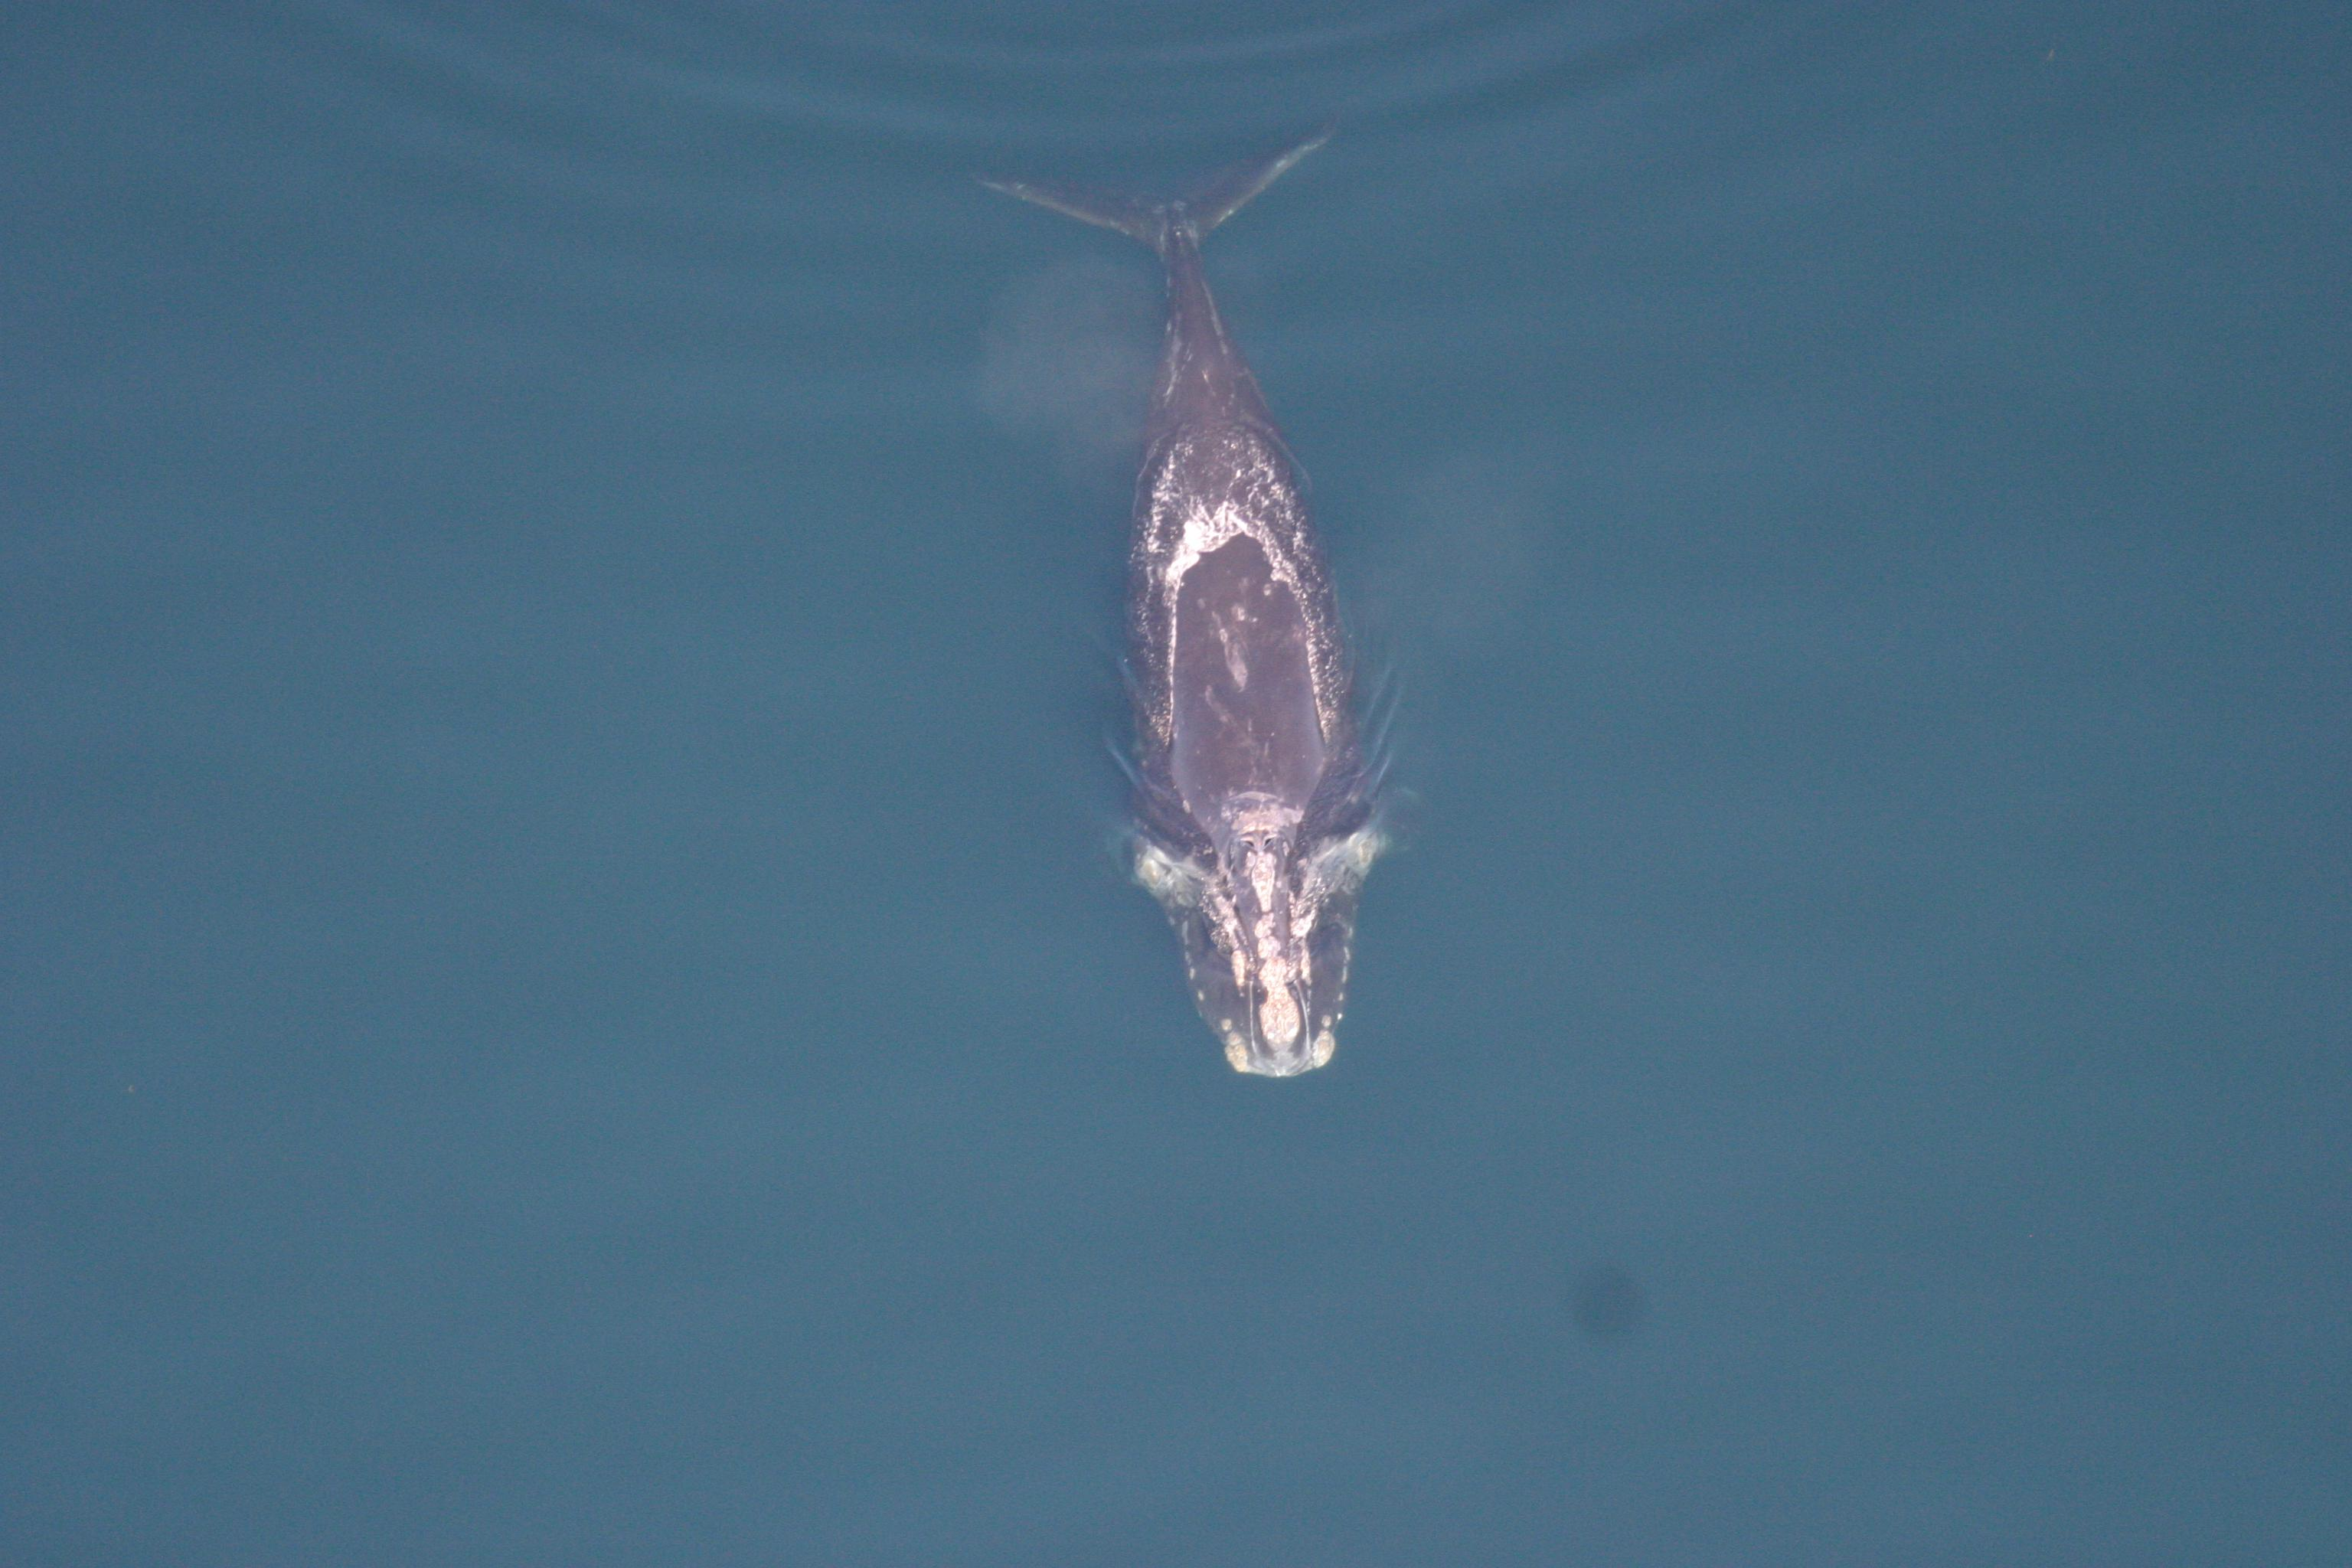
\includegraphics[scale=.25]{example.png}
\caption{Example from data set.}
\end{figure}
\end{frame}

\begin{frame}{Data Example}
\begin{figure}
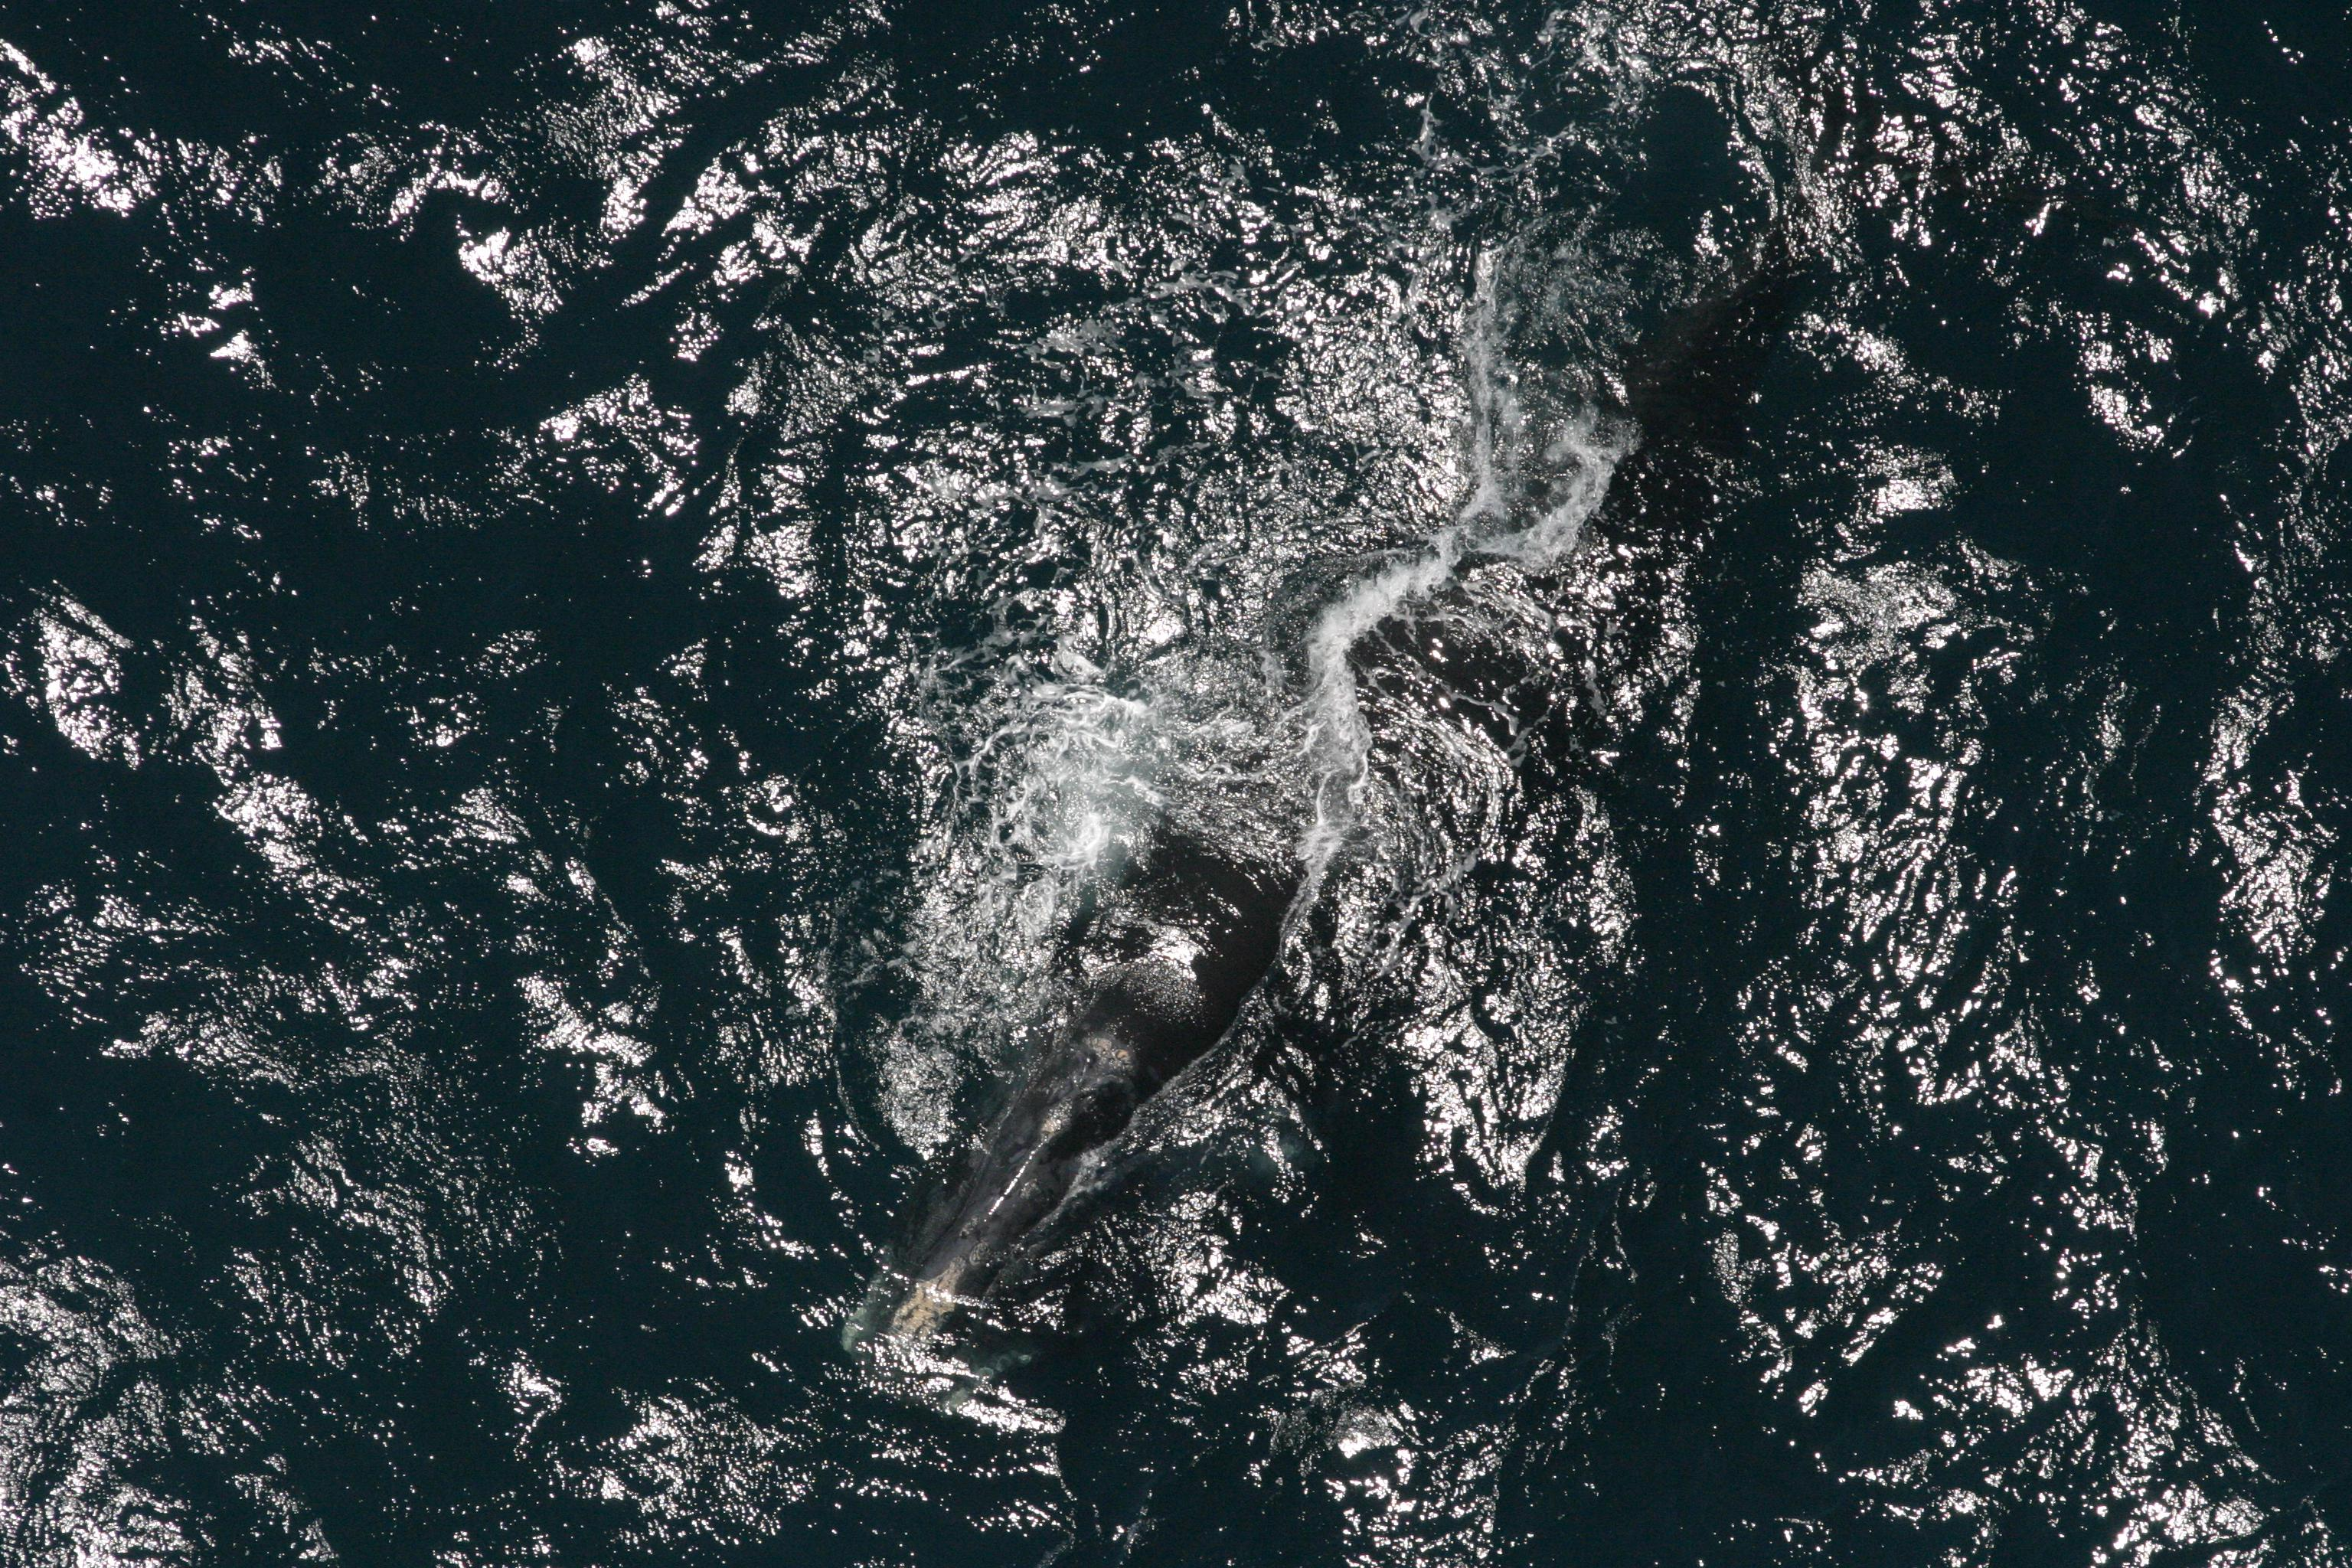
\includegraphics[scale=.25]{example2.png}
\caption{Different lighting and angle.}
\end{figure}
\end{frame}

\begin{frame}{Noise in Data}
\begin{itemize}
\item Other whales
\item Dolphins
\item Birds
\item Surface reflectivity
\item Dirty/clouded water
\end{itemize}
\end{frame}

\begin{frame}{Training Data}
\begin{itemize}
\item List of photos with whale ID provided
\item Label whales by hand to teach recognizer.
\end{itemize}
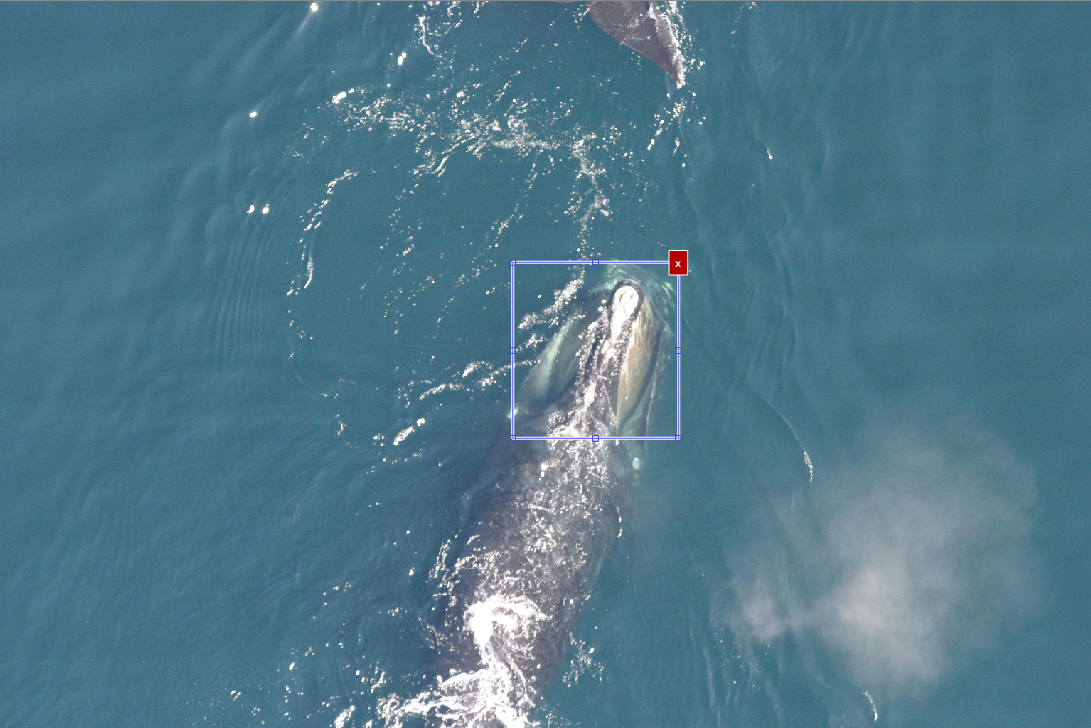
\includegraphics[scale=.25]{label.png}
\end{frame}

\begin{frame}{Matlab Cascade Object Detector}
\begin{itemize}
\item Machine learning tool
\item Trains in stages
\item Requires positive and negative examples
\end{itemize}
\end{frame}

\begin{frame}{Matlab Cascade Object Detector}
Parameters:
\begin{itemize}
\item Number of Training stages
\item False Alarm Rate
\end{itemize}
\end{frame}

\begin{frame}{Results}
\begin{figure}
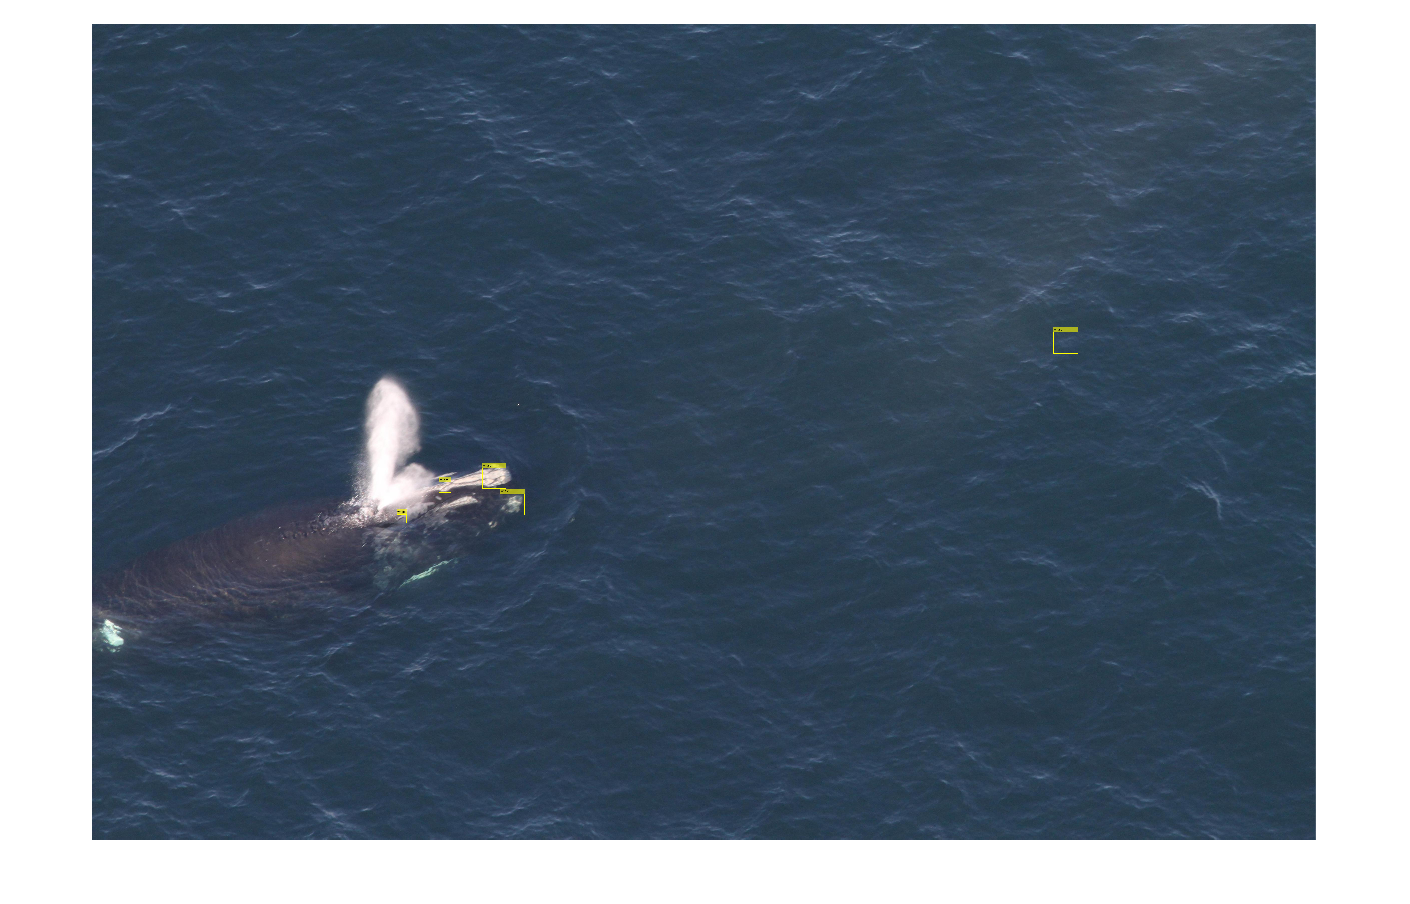
\includegraphics[scale=.25]{recog.png}
\end{figure}
\end{frame}

\section{Identification}
\subsection{Identification}
\begin{frame}{Approaches}
\begin{itemize}
\item Neural Network
\item Deep-Belief Network
\end{itemize}
\end{frame}

\begin{frame}{References}
\bibliography{project.bib}
\nocite{*}
\end{frame}

\end{document}
